\documentclass{standalone}
\usepackage{graphicx}	
\usepackage{amssymb, amsmath, amsthm}
\usepackage{color}

\usepackage{tikz}
\usetikzlibrary{math, calc, arrows.meta}

\definecolor{light}{RGB}{220, 188, 188}
\definecolor{mid}{RGB}{185, 124, 124}
\definecolor{dark}{RGB}{143, 39, 39}
\definecolor{highlight}{RGB}{180, 31, 180}
\definecolor{gray10}{gray}{0.1}
\definecolor{gray20}{gray}{0.2}
\definecolor{gray30}{gray}{0.3}
\definecolor{gray40}{gray}{0.4}
\definecolor{gray60}{gray}{0.6}
\definecolor{gray70}{gray}{0.7}
\definecolor{gray80}{gray}{0.8}
\definecolor{gray90}{gray}{0.9}
\definecolor{gray95}{gray}{0.95}


\begin{document}

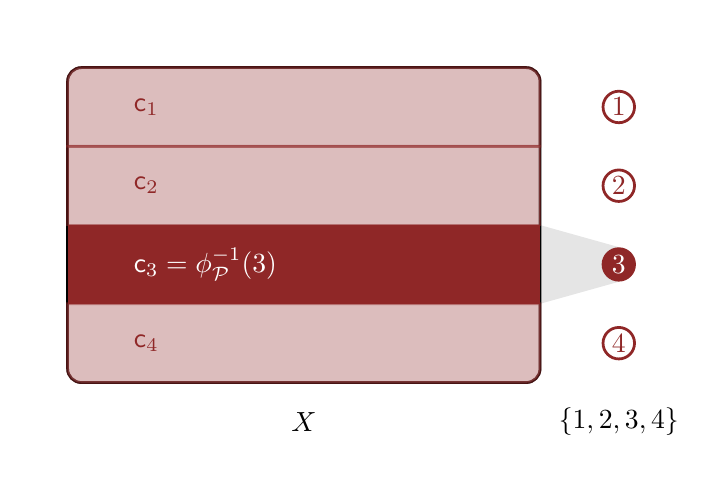
\begin{tikzpicture}[scale=1]
  \draw[white] (-0.5, -1) rectangle (8, 4.5);
  
  \fill[gray90] (6, 1) -- (7, 1.28) -- (7, 1.72) -- (6, 2) -- cycle;
  
  \draw[rounded corners=5, color=black, line width=1] (0, 0) rectangle (6, 4);
  \node at (3, -0.5) { $X$ };
  
  \filldraw[draw=dark, fill=mid, opacity=0.5, line width=1]
    (0, 3) -- (6, 3) {[rounded corners=5] -- (6, 4) -- (0, 4)} -- cycle;
  \node[dark] at (1, 3.5) { $\mathsf{c}_{1}$ };

  \filldraw[draw=dark, fill=mid, opacity=0.5, line width=1]
    (0, 2) -- (6, 2) -- (6, 3) -- (0, 3) -- cycle;
  \node[dark] at (1, 2.5) { $\mathsf{c}_{2}$ };
        
  \filldraw[draw=dark, fill=mid, opacity=0.5, line width=1]
    (0, 1) -- (6, 1) {[rounded corners=5] -- (6, 0) -- (0, 0)} -- cycle;
  \node[dark] at (1, 0.5) { $\mathsf{c}_{4}$ };

  \foreach \i in {1, 2, 3, 4} {
    \draw[dark, line width=1] (7, 3.5 + 1 - \i) circle (0.2);
    \node[dark] at (7, 3.5 + 1 - \i) { $\i$ };
  }
  
  \fill[dark, line width=1] (7, 3.5 + 1 - 3) circle (0.2);
  \node[white] at (7, 3.5 + 1 - 3) { $3$ };
  
  \fill[dark, line width=1] (0, 1) -- (6, 1) -- (6, 2) -- (0, 2) -- cycle;
  \node[white] at (1.75, 1.5) { $\mathsf{c}_{3} = \phi_{\mathcal{P}}^{-1}(3)$ };
  
  \node at (7, -0.5) { $\{1, 2, 3, 4\}$ };

  
  

\end{tikzpicture}

\end{document}  